%%
% The BIThesis Template for Bachelor Graduation Thesis
%
% 北京理工大学毕业设计(论文)第一章节 —— 使用 XeLaTeX 编译
%
% Copyright 2020 Spencer Woo
%
% This work may be distributed and/or modified under the
% conditions of the LaTeX Project Public License, either version 1.3
% of this license or (at your option) any later version.
% The latest version of this license is in
%   http://www.latex-project.org/lppl.txt
% and version 1.3 or later is part of all distributions of LaTeX
% version 2005/12/01 or later.
%
% This work has the LPPL maintenance status maintained'.
%
% The Current Maintainer of this work is Spencer Woo.
%
% 第三章节
\chapter{基于GeoHash的地图信息存储}
车辆位置信息和地图信息在路由和安全应用中发挥着重要作用。攻击者可以通过位置欺骗达到利己的目的。利用区块链特性,方便多车辆协作,防止数据篡改,为位置信息等提供安全性保障。在本章中,将介绍如何将地图数据处理为GeoHash编码,并实现区域绑定,最终将其存入区块链上。

\section{相关技术}
\subsection{GeoHash编码}
GeoHash是一种新型的地址编码方式,由 Gustavo Niemeyer 和 G.M. Morton发明\cite{lposition},其具体算法是二分法结合编码的一种地理位置信息算法\cite{liu2014geohash},被广泛应用到地理位置表示中。最开始,以本初子午线、赤道为界,地球可以分为4个部分,设定西经为负,南纬为负,所以地球上的经度范围就是[-180,180],纬度范围就是[-90,90]。经纬度的二进制码也是通过二分来进行确认的,以(116.3639092,39.9662639)为例,经纬度转为二进制编码,GeoHash精度为8,过程如下表\ref{经纬度计算}所示。

\begin{table}[!ht]
  \centering
  \caption{经纬度计算}
  \label{经纬度计算}
  \subcaption*{Table1 经度计算}
  \begin{tabular}{*{5}{>{\centering\arraybackslash}p{3cm}}}
  \hline
         &  经度范围             & 划分区间(0)           & 划分区间(1)            &  116.3639092   \\ \hline
    1    &  (-180,180)         & (-180,0)             & (0,180)              & 1  \\
    2    & 	(0,180)            & (0,90)               & (90,180)             & 1  \\
    3    & 	(90,180)           & (90,135)             & (135,180)            & 0  \\ 
    4    & (90,135)            & (90,112.5)            & (112.5,135)           & 1 \\ 
    5    & (112.5,135)          &	(112.5,123.75)        & 	(123.75,135)        & 0 \\ 
    6    & (112.5,123.75)       & (112.5,118.125)      & (118.125,123.75)      & 0 \\ 
    7    & (112.5,118.125)     & (112.5,115.3125)     & (115.3125,118.125)    & 	1 \\ 
    8    & (115.3125,118.125)	& (115.3125,116.71875) & (116.71875,118.125)	 & 	0 \\ 
    \hline
    \end{tabular}
  \bigskip
  \subcaption*{Table2 纬度计算}
  \begin{tabular}{*{5}{>{\centering\arraybackslash}p{3cm}}}
    \hline
           & 纬度范围    & 划分区间(0)    & 划分区间(1)   &  39.9662639   \\ \hline
    1    & (-90,90)  & 	(-90,0) & (0,90)  & 1  \\
    2   & 	(0,90)  & (0,45)  & (45,90)  & 0  \\
    3 & 	(0,45)  & (0,22.5)  & (22.5,45)  & 1  \\ 
    4    & 	(22.5,45) & 	(22.5,33.75) & (33.75,45) & 1 \\ 
    5    & (33.75,45) &		(33.75,39.375) & (39.375,45) & 1 \\ 
    6    & (39.375,45) & (39.375,42.1875) & (42.1875,45) & 0 \\ 
    7    & (39.375,42.1875) & (39.375,40.78125) & (40.78125,42.1875)	 & 	0 \\ 
    8    & 	(39.375,40.78125)	 & 	(39.375,40.078125) & (40.078125,40.78125)	 & 	0 \\ 
    \hline
    \end{tabular}
\end{table}

将经度和纬度分别转换成一组二进制字符串,然后将经度和纬度的二进制字符串交叉结合成一组新的二进制字符串,新的二进制字符串中对应偶数位的序列是经度序列,对应奇数位的序列是纬度序列,然后将新字符串转为十进制并根据Base32(即数字0-9和字母b-z不包括a,i,l,o的32个字符)进行编码\cite{liu2014geohash},最终实现用一维数据表示二维数据的效果。

Geohash特殊的编码方式,一个GeoHash值对应一个近似矩形的覆盖区域,当位数较少时,它可以表示一块区域的坐标,当位数足够长时,它可以表示地球上某个具体点的坐标,而且,位数短的区域一定包含以此为前缀的地图数据,对地图数据进行区域绑定提供了极大的便利。GeoHash在编码过程中保留了一定的相对地理位置信息,在大部分情况下,GeoHash编码共同前缀越长的区块物理距离越近\cite{lposition}。

传统的地图数据采用经纬度的方法进行存储,不方便实现位置与区域绑定,采用GeoHash字符串存储地图信息可以使所有信息平面化,避免使用树状结构,更方便区域信息绑定,也更适用于Solidity语言特性。同时,根据GeoHash编码规则,一个GeoHash值所代表的区域一定包含以该GeoHash值为前缀的所有元素。

\subsection{区块链}
区块链具有去中心化、分布式、点对点、集体维护等特点,其上交易的不可更改性保证了数据的可靠性,通过编写智能合约,将地图数据存入区块链,可以使得移动端用户获取安全正确的数据,且稳定性更高,更有利于车载终端互连。

\subsection{Web3Js}
前端使用web3js-v1.2.29调用,首先需要Web3.providers.HttpProvider绑定监测IP:
\begin{center}
  \fbox{
    web3Map = new Web3(new Web3.providers.HttpProvider(mapContractServer));
  }
\end{center}

然后使用eth.Contract绑定对应合约,其中mapContractAbi是合约接口,mapContractAddress是合约部署到区块链上的地址:
\begin{center}
  \fbox{
    mapContract = new web3Map.eth.Contract(mapContractAbi,mapContractAddress);	
  }
\end{center}

在与合约进行交易的时候,需要调用methods下的call和send方法,如果是发送交易,需要更改区块链数据则调用send方法:
\begin{center}
  \fbox{
    \parbox{130mm}{
    trafficContract.methods.setSlingePos(userId, locTime[index], latOri, lonOri, latFix, lonFix).send(
    \{from: trafficContractAccount, gas: 500000\});
    }
  }
\end{center}

如果是获取区块链上的数据则使用call方法:
\begin{center}
  \fbox{
    \parbox{130mm}{
      trafficContract.methods.getQuality(userId).call(function(error, result)\{
      \par if(!error) \{
      \par      console(result);
      \par          \} else
      \par    console.error(error);
      \});
    }
    }
\end{center}

\section{实现思路}
\subsection{数据转换}
原始数据为GeoJson的经纬度格式,如下:

(1) 点:
\begin{center}
  \fbox{
    \parbox{130mm}{
      \{"type":"Feature","geometry":\{"type":"Point","coordinates":[116.3639092,\par 39.9662639]\},"properties":\{"highway":"traffic\_signals","name":"name"\par \}\}
    }
  }
\end{center}

(2) 道路:
\begin{center}
  \fbox{
    \parbox{130mm}{
      \{"type":"Feature","geometry":\{"type":"LineString","coordinates":[[\par 116.3894407, 39.9062721],[116.3894463,39.9060115]]\},\par "properties":\{"highway":"primary","name":"广场西侧路",\par "oneway":"yes"\}\}
    }
  }
\end{center}

(3) 建筑物:
\begin{center}
  \fbox{
    \parbox{130mm}{
      \{"type":"Feature","geometry":\{"type":"MultiPolygon","coordinates":[[[[\par 116.390632,39.9165908],[116.3906404,39.9163544],[116.3908015,\par 39.9163577],[116.3909492,39.9163608],[116.3909408,39.9165972],\par [116.3907829,39.9165939],[116.390632,39.9165908]]]]\},"properties":\{ \par "building":"yes","name":"中和殿"\}\}
    }
  }
\end{center}

编写JS脚本将对应坐标数据转化为GeoHash编码:

(1) 点:
\begin{center}
  \fbox{
    \parbox{130mm}{
      \{"type":"Feature","geometry":\{"type":"Point","coordinates":["wx4ergts7ee" \par ]]\},"properties":\{"highway":"traffic\_signals","name":"name"\par \}\}
    }
  }
\end{center}

(2) 道路:
\begin{center}
  \fbox{
    \parbox{130mm}{
      \{"type":"Feature","geometry":\{"type":"LineString","coordinates":[[ \par "wx4g088nys3","wx4g088jqet"]\},"properties":\{"highway":"primary" \par ,"name":"广场西侧路","oneway":"yes"\}\}
    }
  }
\end{center}

(3) 建筑物:
\begin{center}
  \fbox{
    \parbox{130mm}{
      \{"type":"Feature","geometry":\{"type":"MultiPolygon","coordinates":[[[ \par 'wx4g0d94frc','wx4g0d91d7z','wx4g0d91whr','wx4g0d939sy', \par 'wx4g0d9713p','wx4g0d95jb6','wx4g0d94frc']]]\},"properties":\{ \par "building":"yes","name":"中和殿"\}\}
    }
  }
\end{center}

\subsection{绑定方法}
在存储地图时,本文将地图划分为精度较低、范围较广的GeoHash块,并实现对应区域中元素与GeoHash块一一绑定,因此想要请求某一区域的地图信息时,只需要通过该区域对应的GeoHash编码值查找。完整的地图数据主要有三种元素:点,道路,建筑物。

在进行绑定时,点只需要绑定到前缀所代表的区域上,根据GeoHash编码规则,3区域的红色点的GeoHash值一定是红色点的前缀,本课题中,通过直接绑定前缀即可绑定区域,如图\ref{点绑定区域}。
\begin{figure}[!htb]
    \centering
    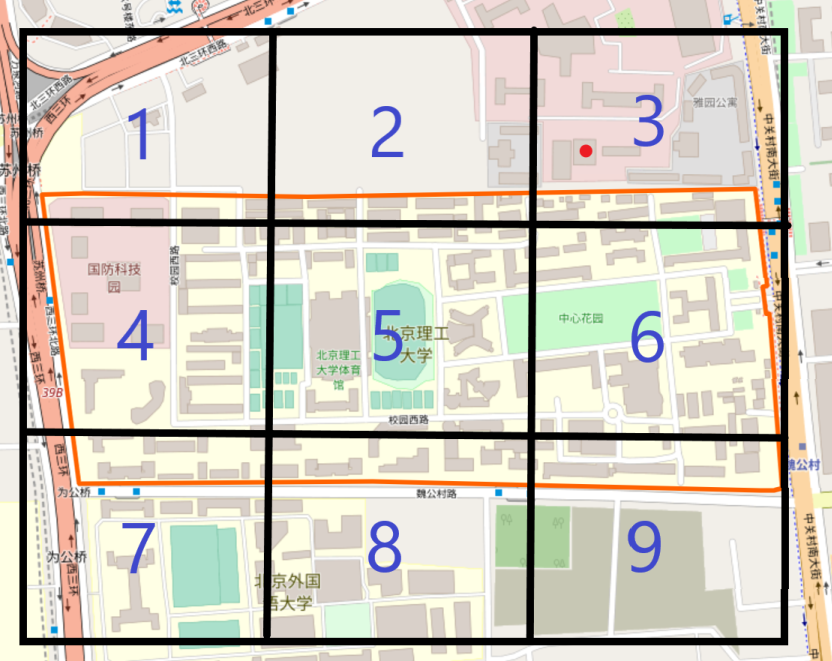
\includegraphics[width=4in]{images/3.png}
    \caption{点绑定区域}\label{点绑定区域} % label 用来在文中索引
\end{figure}

对于道路,地图数据中以矢量的形式出现,取其起点和终点,将其当作一条直线,对于经纬度,0.01°经度代表1000m,0.01°纬度代表1113m,所以通过遍历从起点到终点的经纬度,以0.01°为间隔,划分出对应区域,然后通过前缀判断与路径上的点是否有交叉,从而判断该直线是否在该区域内。如图\ref{道路绑定区域},红色路径经过区域4和区域7,通过上述遍历,可以划分出直线所经过的区域编码,如果该路径存在点在区域4中,则属于区域4,同理,如果存在点在区域7中,则属于区域7。
\begin{figure}[H]
    \centering
    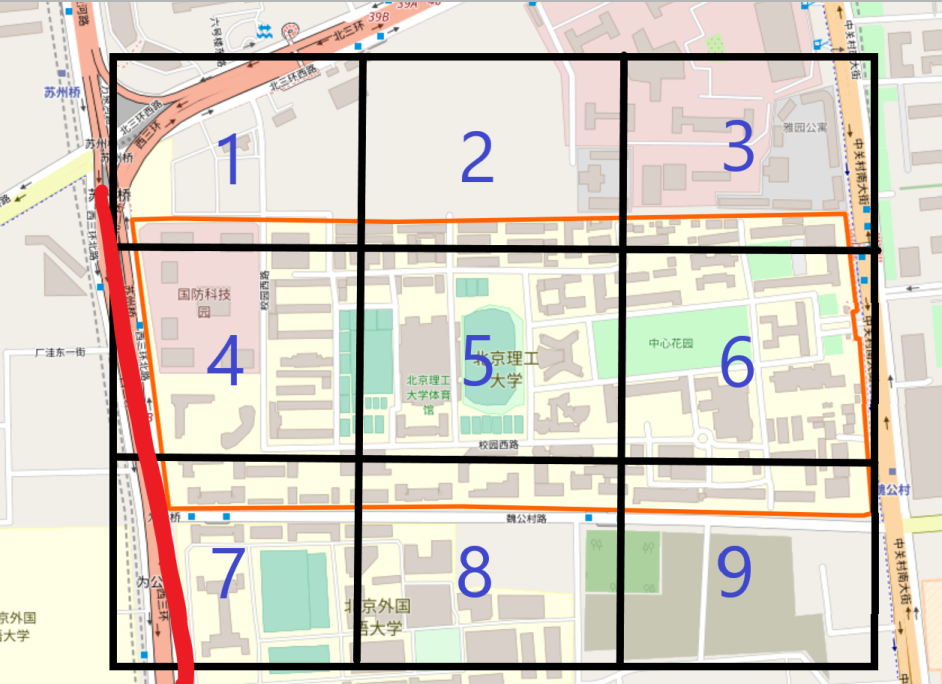
\includegraphics[width=4in]{images/4.png}
    \caption{道路绑定区域}\label{道路绑定区域} % label 用来在文中索引
  \end{figure}

对于建筑物,地图数据中建筑物是多边形数据,且建筑物一般横跨区域不大,所以通过遍历多边形上的点元素,将其绑定到前缀所对应的区域上,即可完成建筑物绑定。如图\ref{建筑物绑定区域},图中中心花园区域横跨两个区域,可通过对应路径前缀进行绑定。
\begin{figure}[H]
    \centering
    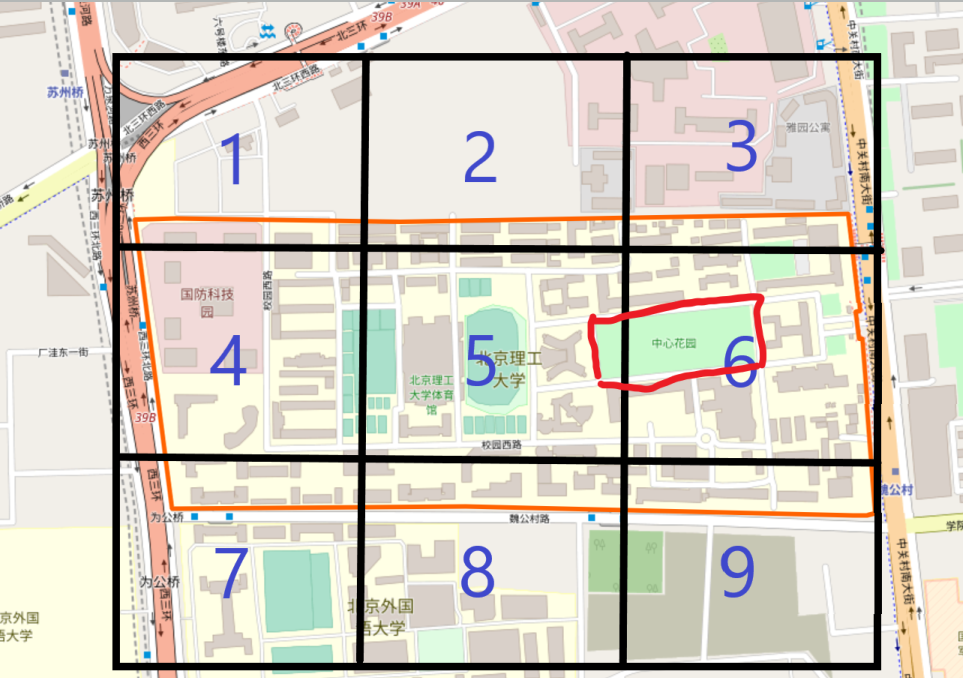
\includegraphics[width=4in]{images/5.png}
    \caption{建筑物绑定区域}\label{建筑物绑定区域} % label 用来在文中索引
  \end{figure}
\subsection{地图存储合约}
合约里面,首先构建了存储一条地图信息的结构体,如图\ref{地图信息结构体}:
\begin{figure}[H]
  \centering
  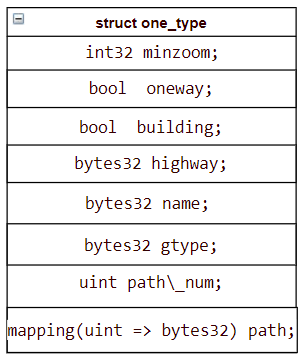
\includegraphics[width=2in]{images/16.png}
  \caption{地图信息结构体}\label{地图信息结构体} % label 用来在文中索引
\end{figure}

对于每条地图数据会有对应的gid编号,通过mapping完成区域与区域内信息的映射。

地图存储合约算法如下:
\begin{algorithm}[H]
  \caption{存储合约} %算法的名字
  \begin{algorithmic}[1] %每行显示行号  
      % \Require Array数组,n数组大小  
      \Require minzoom,oneway,building,highway,name,gtype
      \Function {get\_onetype}{gid}  
        \Return {types\_list[gid]}
      \EndFunction  

      \Function {get\_types}{hash} \\ 
          //获取对应geohash区域内所有道路信息 \\ 
          \Return{geo\_maps[hash]}
      \EndFunction  
      \Function {add\_onetype}{gid,minzoom,oneway,building,highway,name,gtype,path}\\  
          //通过id查询信息
          \State  Onetype.minzoom <- minzoom;
          \State  Onetype.oneway <- oneway;
          \State  Onetype.building <- building;
          \State  Onetype.highway <- highway;
          \State  Onetype.name <-name;
          \State  Onetype.gtype <- gtype;
          \State  Onetype.path <- path;
      \EndFunction  
      \Function {add\_area\_line}{hash,gid}  //绑定区域
          \State num <- geo\_maps[hash].num++;
          \State geo\_maps[hash].types\_list[num] <- gid;
      \EndFunction
  \end{algorithmic}  
\end{algorithm}

\section{小结}
本章中,首先对GeoHash编码进行了介绍,阐明了经纬度数据到GeoHash编码的基本逻辑,并简要介绍GeoHash的相关优点。另外,本章完成了将地图的经纬度数据到GeoHash数据的转换,阐明了地图数据区域绑定的基本逻辑,至此地图存储工作完成,后续将通过GeoHashTile前端结合,展现地图效果。